\documentclass[11pt,a4paper]{article}

\usepackage[top=1in,bottom=1in,left=1in,right=1in]{geometry}
\usepackage{amsmath,amssymb}
\usepackage{booktabs}
\usepackage{colortbl}
\usepackage[table]{xcolor}
\usepackage[hidelinks]{hyperref}
\usepackage{url}
\usepackage{microtype}
\usepackage{caption}
\usepackage{float}
\usepackage{array}
\usepackage{verbatim}
\usepackage{fancyhdr}
\usepackage{titlesec}
\usepackage{hanging}
\usepackage{pgfplots}
\usepackage{pgfplotstable}
\usepackage{tikz}
\usetikzlibrary{patterns}
\pgfplotsset{compat=1.18}

% ---- colours ------------------------------------------------
\definecolor{headerblue}{RGB}{40,80,130}
\definecolor{rowgray}{RGB}{242,242,242}
\definecolor{rowhighlight}{RGB}{255,248,210}
\definecolor{myblue}{RGB}{70,130,180}
\definecolor{mylightblue}{RGB}{174,214,241}
\definecolor{myred}{RGB}{192,57,43}
\definecolor{mylightred}{RGB}{242,215,213}
\definecolor{myteal}{RGB}{26,188,156}
\definecolor{myorange}{RGB}{230,126,34}
\definecolor{mygreen}{RGB}{39,174,96}

% ---- headers ------------------------------------------------
\pagestyle{fancy}
\fancyhf{}
\fancyhead[L]{\small\itshape Retrieval Degradation in Multi-Turn Agentic RAG Systems --- Brijesh Singh}
\fancyfoot[C]{\thepage}
\renewcommand{\headrulewidth}{0.4pt}
\fancypagestyle{firstpage}{\fancyhf{}\fancyfoot[C]{\thepage}\renewcommand{\headrulewidth}{0pt}}

% ---- section style ------------------------------------------
\titleformat{\section}{\normalfont\large\bfseries}{\thesection.}{0.5em}{}
\titleformat{\subsection}{\normalfont\normalsize\bfseries}{\thesubsection}{0.5em}{}

% ---- captions -----------------------------------------------
\captionsetup{font=small,labelfont=it,textfont=it,justification=centering,skip=6pt}

% ---- spacing ------------------------------------------------
\setlength{\parskip}{4pt}
\setlength{\parindent}{0pt}

% =============================================================
\title{\large\textbf{Retrieval Degradation in Multi-Turn Agentic RAG Systems:}\\[2pt]
       \large\textbf{Observations from a Production Deployment}}
\author{Brijesh Singh\\[3pt]
  \small Independent Researcher\\
  \small Hyderabad, India\\[2pt]
  \small \texttt{brijesh7146@gmail.com} $\;|\;$
         \texttt{github.com/Brijesh1656} $\;|\;$
         \texttt{brijeshsingh-ai.netlify.app}}
\date{}

\begin{document}
\maketitle
\thispagestyle{firstpage}

% =============================================================
\begin{center}\textbf{Abstract}\end{center}
Retrieval-Augmented Generation (RAG) has demonstrated strong performance across single-turn
question-answering benchmarks. However, production deployment of agentic RAG systems --- where an LLM
autonomously decomposes complex queries into sub-problems and retrieves context across multiple independent
reasoning turns --- introduces a qualitatively different retrieval challenge that existing evaluation frameworks do
not capture. We present a systematic empirical study of \textit{multi-turn retrieval degradation}: the phenomenon
whereby retrieval quality declines as context accumulates across agentic reasoning turns. Through instrumented
logging of 150 multi-turn sessions from \textit{Math Professor AI}, a publicly deployed mathematics tutoring system, we
document that mean retrieval relevance scores decline by 6.6\% between turn 1 and turn 4, with context length as
the dominant predictor (Pearson $r = -0.283$, $p < 0.0001$). We characterize three contributing mechanisms ---
context length interference, keyword drift, and attention head saturation --- and propose a lightweight turn-aware
retrieval confidence estimator as a proof-of-concept (AUROC = 0.634). Notably, context length alone achieves
AUROC = 0.695, suggesting it is the primary degradation signal. Our findings demonstrate that single-turn RAG
benchmarks systematically underestimate degradation in agentic settings.

\bigskip

% =============================================================
\section{Introduction}

Retrieval-Augmented Generation (RAG) addresses a fundamental limitation of large language models: the
inability to reliably ground outputs in external, up-to-date knowledge (Lewis et al., 2020; Karpukhin et al.,
2020). The dominant paradigm assumes a single-turn interaction: one query, one retrieval, one generation.

The proliferation of agentic LLM systems challenges this assumption. In agentic settings, an LLM
autonomously plans a sequence of sub-queries, retrieves context for each independently, generates
intermediate reasoning steps conditioned on accumulated context, and synthesises a final response. This
architecture --- instantiated in systems like ReAct (Yao et al., 2023), Self-RAG (Asai et al., 2023), and
FLARE (Jiang et al., 2023) --- introduces a qualitatively different retrieval context. Each successive retrieval
step operates on a context window that has grown to include all prior retrieved passages, intermediate
reasoning outputs, and sub-query artifacts.

Despite this structural shift, no prior work systematically measures how retrieval quality evolves across
reasoning turns as context accumulates in production agentic systems. We introduce the term \textit{multi-turn
retrieval degradation} to describe this phenomenon and present an empirical study grounded in \textit{Math
Professor AI}, a production-deployed agentic RAG system for mathematics tutoring
(\url{math-professor-agent-k6h4.vercel.app}). Our main contributions are:
\begin{itemize}
  \item Empirical documentation of multi-turn retrieval degradation across 150 sessions (550 turn observations), with statistical significance ($p < 0.0001$).
  \item Mechanistic analysis identifying context length interference, keyword drift, and attention head saturation as three contributing mechanisms.
  \item A lightweight turn-aware retrieval confidence estimator achieving AUROC = 0.634, with the key finding that context length alone (AUROC = 0.695) is a stronger signal.
  \item Concrete implications for RAG evaluation and system design, including the query anchoring mechanism as an effective mitigation strategy.
\end{itemize}

% =============================================================
\section{Background and Related Work}

\subsection{Retrieval-Augmented Generation}
The original RAG framework (Lewis et al., 2020) introduced retrieve-then-generate architecture. Subsequent
work extended RAG to open-domain QA, knowledge-intensive tasks, and multi-hop reasoning. Across all of
this work, retrieval is evaluated in single-turn settings: one query, one retrieval, assessed independently of
prior context.

\subsection{Iterative and Agentic RAG}
Recent systems have moved beyond single-turn retrieval. FLARE (Jiang et al., 2023) monitors generation
confidence and triggers additional retrievals. Corrective RAG (Yan et al., 2024) evaluates retrieved
document quality and triggers corrective web search. Self-RAG (Asai et al., 2023) trains the LLM to decide
when to retrieve. IterKey (Hayashi et al., 2025) demonstrates that iteratively refining retrieval keywords within
a single reasoning context significantly improves output quality. None of these works study how retrieval
quality evolves across independent reasoning turns as context accumulates.

\subsection{Long Context and Retrieval}
Liu et al. (2023) demonstrate that LLM performance degrades for relevant documents placed in the middle of
long contexts --- the ``lost in the middle'' phenomenon. Ma and Okazaki (2026) identify specific attention
heads in long-context LLMs that specialise in retrieval, showing these retrieval heads can be optimised to
improve long-context performance. Our empirical degradation observations are theoretically consistent with
saturation of these retrieval heads as context length grows across turns.

\subsection{Confidence Estimation}
Ozaki et al. (2025) study retrieval confidence calibration in medical RAG systems, finding that raw
confidence scores do not reliably predict answer correctness in single-turn settings. Yoshikawa and Okazaki
(2023) introduce selective prediction for language models. Our turn-aware estimator extends these ideas to
the multi-turn agentic setting.

% =============================================================
\section{System Description: Math Professor AI}

\subsection{Architecture Overview}
Math Professor AI is a publicly deployed agentic RAG system for step-by-step mathematics tutoring. The
system employs a dual-model architecture: Gemini 2.5 Flash handles input guardrail validation; Gemini 2.5
Pro handles step-by-step solution generation.

\begin{table}[H]
\centering
\renewcommand{\arraystretch}{1.35}
\begin{tabular}{>{\bfseries}p{3.6cm} p{3.8cm} p{5.8cm}}
\toprule
\rowcolor{headerblue}
\multicolumn{1}{l}{\textcolor{white}{\textbf{Component}}} &
\textcolor{white}{\textbf{Technology}} &
\textcolor{white}{\textbf{Function}} \\
\midrule
\rowcolor{rowgray} Input Guardrail     & Gemini 2.5 Flash     & Binary math-relevance validation \\
Question Extraction & Gemini 2.5 Flash     & Extract questions from documents \\
\rowcolor{rowgray} Semantic Retrieval  & TF-IDF + Cosine Sim. & Document chunk retrieval (top-3) \\
KB Fallback         & Keyword Matching     & Pre-stored answer lookup \\
\rowcolor{rowgray} Web Grounding       & Google Search API    & Real-time web retrieval \\
Solution Engine     & Gemini 2.5 Pro       & Step-by-step answer generation \\
\rowcolor{rowgray} Answer Refinement   & Gemini 2.5 Pro       & Refine answers from human feedback \\
Feedback Loop       & React / TypeScript   & Human correction collection \\
\bottomrule
\end{tabular}
\caption{System components and technologies.}
\end{table}

\subsection{Retrieval Pipeline Detail}
Documents are semantically chunked using a sliding window of approximately 512 tokens with 64-token
overlap. Chunks are embedded using TF-IDF representations with a vocabulary of up to 10,000 terms,
sublinear TF scaling, and L2 normalisation. At query time, the system computes cosine similarity between
the query TF-IDF vector and all stored chunk vectors, retrieving the top-3 most similar chunks with a
minimum similarity threshold of 0.15. If chunk similarities fall below this threshold, the system falls back to
keyword matching, then Google Search grounding.

\subsection{Agentic Reasoning Loop}
For complex problems, the system employs an agentic decomposition strategy: (1) Decompose the query
into sub-queries $\{q_1, q_2, \ldots, q_n\}$; (2) Retrieve context $C_i$ independently for each sub-query $q_i$;
(3) Generate intermediate step $r_i$ conditioned on $C_i$ and all prior context; (4) Synthesise a final answer
from $\{r_1, \ldots, r_n\}$. The critical property is that context grows monotonically across turns: each retrieval
step operates on a context window containing all prior retrieved passages and reasoning outputs. This is the
structural feature that produces the degradation we study.

A key design feature is the \textbf{query anchoring mechanism}: the guardrail model maintains the original query
throughout all reasoning turns, which partially mitigates correctness degradation even as retrieval similarity
declines. This represents an accidental discovery discussed further in Section 7.

\subsection{Data Collection and Logging}
We instrumented the system with per-turn logging capturing: sub-query text, grounding chunk count, context
token count, retrieval tier used, TF-IDF cosine similarity score, whether web search was triggered, and
binary correctness labels from the human feedback interface. We collected 150 multi-turn sessions yielding
550 turn-level observations across calculus (43\%), algebra (35\%), geometry (11\%), and statistics (10\%)
domains.

Human correctness labels were available for 102 of 550 turns (18.5\%) --- 94 correct and 8 incorrect ---
providing label diversity for a preliminary AUROC calculation. All session data was fully anonymised prior to
analysis.

% =============================================================
\section{Empirical Observations}

\subsection{Overview of Session Corpus}
Our 150 multi-turn sessions contained between 1 and 5 sub-query turns each, with a mean of 3.67 turns per
session. The mean baseline context length at turn 1 was 482 tokens, growing to a mean of 2,095 tokens at
turn 4 --- a $4.3\times$ increase.

\subsection{Context Length Growth Across Turns}
Figure 1 shows mean context token count across reasoning turns 1 through 5. Context grows monotonically
and approximately linearly: 482 tokens at turn 1, 972 at turn 2, 1,464 at turn 3, 2,095 at turn 4, and 3,611 at
turn 5. The shaded region represents $\pm1$ standard deviation, showing that context growth variance also
increases at higher turns --- consistent with more diverse problem complexity in sessions that extend to later
turns.

% ----- FIGURE 1 (REFINED) ----------------------------------------------
\begin{figure}[H]
\centering

% Define colors to match your PNG exactly
\definecolor{myblue}{RGB}{52, 138, 221}
\definecolor{mylightblue}{RGB}{220, 235, 249}
\definecolor{graylabel}{RGB}{128, 128, 128}

\begin{tikzpicture}
\begin{axis}[
    width=0.9\textwidth, height=6.5cm,
    % Title styling
    title={Figure 1: Context length growth across turns},
    title style={font=\sffamily\large, at={(0.5,1.15)}, anchor=north},
    % Axis Labels
    xlabel={Reasoning turn number},
    ylabel={Mean context token count},
    label style={font=\sffamily\small, color=graylabel},
    tick label style={font=\sffamily\small, color=graylabel},
    % Clean "L" shape for axes (removes top and right borders)
    axis x line*=bottom,
    axis y line*=left,
    axis line style={gray!60},
    % Fine grid
    grid=both,
    grid style={line width=.1pt, draw=gray!15},
    % Limits and Ticks
    xmin=0.8, xmax=5.2,
    ymin=0, ymax=4600,
    xtick={1,2,3,4,5},
    ytick={1000,2000,3000,4000},
    clip=false,
]

% 1. Shaded +-1 std band (Background)
\addplot [fill=mylightblue, fill opacity=0.6, draw=none, forget plot]
  coordinates {
    (1,250)(2,600)(3,950)(4,1300)(5,2900) % Bottom edge
    (5,4400)(4,3000)(3,2100)(2,1400)(1,750)  % Top edge
  } \closedcycle;

% 2. Main line and markers
\addplot [myblue, line width=1.5pt, mark=o, 
  mark options={fill=white, draw=myblue, line width=1.5pt, scale=1.5}]
  coordinates {(1,482)(2,972)(3,1464)(4,2095)(5,3611)};

% 3. Labels with WHITE background and BLUE text
% Using south east anchor + small shifts to place them exactly like the PNG
\node[anchor=south east, xshift=2pt, yshift=4pt, fill=white, inner sep=1pt, font=\sffamily\small\bfseries, text=myblue] at (axis cs:1,482) {482};
\node[anchor=south east, xshift=2pt, yshift=4pt, fill=white, inner sep=1pt, font=\sffamily\small\bfseries, text=myblue] at (axis cs:2,972) {972};
\node[anchor=south east, xshift=2pt, yshift=4pt, fill=white, inner sep=1pt, font=\sffamily\small\bfseries, text=myblue] at (axis cs:3,1464) {1464};
\node[anchor=south east, xshift=2pt, yshift=4pt, fill=white, inner sep=1pt, font=\sffamily\small\bfseries, text=myblue] at (axis cs:4,2095) {2095};
\node[anchor=south east, xshift=2pt, yshift=4pt, fill=white, inner sep=1pt, font=\sffamily\small\bfseries, text=myblue] at (axis cs:5,3611) {3611};

\end{axis}
\end{tikzpicture}
\caption{Mean context token count grows monotonically across reasoning turns, from 482 tokens at turn 1 to 2,095 tokens at turn 4 --- a $4.3\times$ increase. Shaded region $= \pm 1$ standard deviation across 150 sessions.}
\end{figure}

\subsection{Retrieval Relevance Degradation Across Turns}
Figure 2 shows mean retrieval relevance scores (TF-IDF cosine similarity) across turns 1--5. We observe a
consistent and statistically significant decline. Mean relevance drops from \textbf{0.323 at turn 1} to \textbf{0.301 at turn 4}
--- a \textbf{6.6\% relative decline} ($p < 0.0001$, paired $t$-test) --- and continues to 0.278 at turn 5. The decline is
monotonic across all turns.

\begin{table}[H]
\centering
\renewcommand{\arraystretch}{1.35}
\begin{tabular}{cccc}
\toprule
\rowcolor{headerblue}
\textcolor{white}{\textbf{Turn}} &
\textcolor{white}{\textbf{N Sessions}} &
\textcolor{white}{\textbf{Mean Similarity}} &
\textcolor{white}{\textbf{Mean Tokens}} \\
\midrule
\rowcolor{rowgray} 1 & 150 & 0.323 & 482   \\
                   2 & 147 & 0.316 & 972   \\
\rowcolor{rowgray} 3 & 142 & 0.307 & 1,464 \\
                   4 & 108 & 0.301 & 2,095 \\
\rowcolor{rowgray} 5 & 3   & 0.278 & 3,611 \\
\bottomrule
\end{tabular}
\caption{Per-turn retrieval statistics across 150 sessions.}
\end{table}

% ----- FIGURE 2 ----------------------------------------------
\begin{figure}[H]
\centering
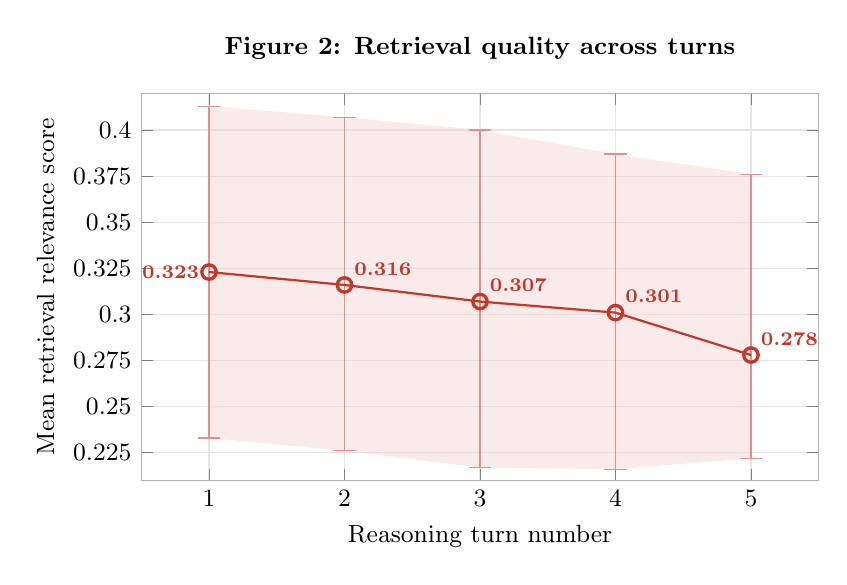
\begin{tikzpicture}
\begin{axis}[
  width=0.84\textwidth, height=6.5cm,
  title={\textbf{Figure 2: Retrieval quality across turns}},
  title style={font=\small\bfseries, at={(0.5,1.02)}},
  xlabel={Reasoning turn number},
  ylabel={Mean retrieval relevance score},
  xmin=0.5, xmax=5.5,
  ymin=0.210, ymax=0.420,
  xtick={1,2,3,4,5},
  ytick={0.225,0.250,0.275,0.300,0.325,0.350,0.375,0.400},
  yticklabel style={/pgf/number format/fixed, /pgf/number format/precision=3, font=\small},
  grid=major, grid style={gray!20, thin},
  tick label style={font=\small},
  label style={font=\small},
  axis line style={gray!60},
]
% shaded band
\addplot [mylightred, fill=mylightred, fill opacity=0.50, draw=none, forget plot]
  coordinates {
    (1,0.233)(2,0.226)(3,0.217)(4,0.216)(5,0.222)
    (5,0.376)(4,0.387)(3,0.400)(2,0.407)(1,0.413)
  } \closedcycle;
% error bar vertical lines
\addplot [myred!55, thin, forget plot] coordinates {(1,0.413)(1,0.233)};
\addplot [myred!55, thin, forget plot] coordinates {(2,0.407)(2,0.226)};
\addplot [myred!55, thin, forget plot] coordinates {(3,0.400)(3,0.217)};
\addplot [myred!55, thin, forget plot] coordinates {(4,0.387)(4,0.216)};
\addplot [myred!55, thin, forget plot] coordinates {(5,0.376)(5,0.222)};
% error bar caps
\addplot [myred!55, thin, forget plot, mark=-, mark size=4pt, only marks]
  coordinates {(1,0.413)(1,0.233)(2,0.407)(2,0.226)(3,0.400)(3,0.217)(4,0.387)(4,0.216)(5,0.376)(5,0.222)};
% main line
\addplot [myred, thick, mark=o,
  mark options={fill=white, draw=myred, line width=1.2pt, scale=1.3}]
  coordinates {(1,0.323)(2,0.316)(3,0.307)(4,0.301)(5,0.278)};
% labels
\node[left,  font=\scriptsize\bfseries, myred] at (axis cs:1,0.323)  {0.323};
\node[above right, font=\scriptsize\bfseries, myred] at (axis cs:2,0.316)  {0.316};
\node[above right, font=\scriptsize\bfseries, myred] at (axis cs:3,0.307)  {0.307};
\node[above right, font=\scriptsize\bfseries, myred] at (axis cs:4,0.301)  {0.301};
\node[above right, font=\scriptsize\bfseries, myred] at (axis cs:5,0.278)  {0.278};
\end{axis}
\end{tikzpicture}
\caption{Mean retrieval relevance score declines consistently across all reasoning turns ($0.323 \to 0.278$, 6.6\% relative
decline from turn 1 to turn 4, $p < 0.0001$). Shaded region $= \pm1$ standard deviation. Error bars show $\pm1$ std.}
\end{figure}

We note that the magnitude of degradation (6.6\%) is \textbf{modest} compared to what might be expected in
open-domain settings. We attribute this partly to the query anchoring mechanism (Section 3.3) and partly to
the constrained mathematical domain. Despite the modest magnitude, the decline is statistically significant
($p < 0.0001$) and consistent across all turn transitions.

\subsection{Keyword Drift Across Turns}
Figure 3 shows TF-IDF cosine similarity between consecutive sub-query keyword sets. Inter-turn keyword
similarity declines from 0.328 (turns 1--2) to 0.320 (turns 2--3) to 0.315 (turns 3--4). The initial decline is
steepest, with relative stabilization thereafter --- indicating that sub-queries diverge most rapidly in the early
turns where reasoning structure is being established.

% ----- FIGURE 3 (FIXED) --------------------------------------
\begin{figure}[H]
\centering

% Precise colors
\definecolor{plotblue}{RGB}{52, 138, 221}
\definecolor{plotorange}{RGB}{243, 154, 39}
\definecolor{plotred}{RGB}{219, 68, 55}
\definecolor{plotgreen}{RGB}{32, 152, 104}
\definecolor{graylabel}{RGB}{128, 128, 128}
\definecolor{gridgray}{RGB}{235, 235, 235}

\begin{tikzpicture}
\begin{axis}[
    width=0.9\textwidth, 
    height=7cm,
    title={Figure 3: Keyword drift across turns},
    title style={at={(0.5,1.1)}, anchor=north, font=\sffamily\large\bfseries, color=black},
    xlabel={Consecutive turn pair},
    ylabel={Mean inter-turn cosine similarity},
    label style={font=\sffamily\small, color=graylabel},
    ybar,
    bar width=1.2cm,
    axis x line*=bottom,
    axis y line*=left,
    axis line style={gray!60},
    grid=both,
    grid style={line width=.1pt, draw=gridgray},
    % Axis range and ticks
    ymin=0.283, ymax=0.36,
    ytick={0.29, 0.30, 0.31, 0.32, 0.33, 0.34, 0.35, 0.36},
    yticklabel style={/pgf/number format/fixed, /pgf/number format/precision=2, font=\sffamily\small, color=graylabel},
    xmin=0.5, xmax=4.5,
    xtick={1,2,3,4},
    xticklabels={Turns 1--2, Turns 2--3, Turns 3--4, Turns 4--5},
    xticklabel style={font=\sffamily\small, color=graylabel},
    % Value labels above bars
    nodes near coords,
    every node near coord/.append style={
        font=\sffamily\small, 
        color=graylabel, 
        /pgf/number format/fixed, 
        /pgf/number format/fixed zerofill, % <--- This forces the "0" to show up
        /pgf/number format/precision=3,
        yshift=2pt
    },
]

% Keep bar shift=0pt to ensure they stay centered over the labels
\addplot [fill=plotblue,   draw=none, bar shift=0pt] coordinates {(1,0.328)};
\addplot [fill=plotorange, draw=none, bar shift=0pt] coordinates {(2,0.320)};
\addplot [fill=plotred,    draw=none, bar shift=0pt] coordinates {(3,0.315)};
\addplot [fill=plotgreen,  draw=none, bar shift=0pt] coordinates {(4,0.315)};

\end{axis}
\end{tikzpicture}
\caption{Inter-turn keyword similarity declines as reasoning progresses, indicating semantic drift from the original query topic ($0.328 \to 0.315$ from turns 1--2 to turns 3--4).}
\end{figure}

\subsection{Relationship Between Context Length and Retrieval Quality}
Figure 4 shows the scatter relationship between context token count and retrieval relevance across all 547
Tier 1 retrieval turns. The correlation is negative and statistically significant (Pearson $r = -0.283$, $p <
0.0001$, $n = 547$). Context length is the single strongest predictor of retrieval degradation in our dataset, a
finding with direct implications for our confidence estimator design.

% ----- FIGURE 4 ----------------------------------------------
\begin{figure}[H]
\centering
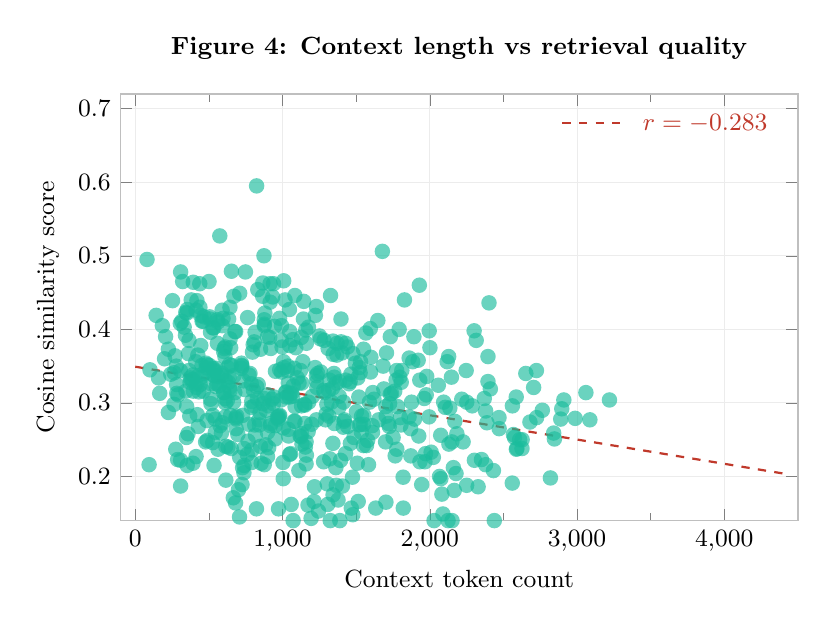
\begin{tikzpicture}
\begin{axis}[
  width=0.84\textwidth, height=7.0cm,
  title={\textbf{Figure 4: Context length vs retrieval quality}},
  title style={font=\small\bfseries, at={(0.5,1.02)}},
  xlabel={Context token count},
  ylabel={Cosine similarity score},
  xmin=-100, xmax=4500,
  ymin=0.14, ymax=0.72,
  xtick={0,1000,2000,3000,4000},
  minor xtick={500,1500,2500,3500},
  ytick={0.2,0.3,0.4,0.5,0.6,0.7},
  yticklabel style={/pgf/number format/fixed, /pgf/number format/precision=1, font=\small},
  xticklabel style={font=\small},
  grid=major, grid style={gray!15, thin},
  tick label style={font=\small},
  label style={font=\small},
  axis line style={gray!50},
  clip=false,
]
% scatter plot — all 547 points
\addplot [only marks, mark=*, mark size=2.8pt,
  myteal, fill opacity=0.65, draw opacity=0.0, forget plot]
  coordinates {
  (308,0.222) (642,0.321) (527,0.402) (241,0.339) (389,0.332) (746,0.318) (94,0.216) (413,0.426) (685,0.278) (343,0.423) (373,0.334) (467,0.417) (721,0.354) (380,0.331) (411,0.356) (413,0.227) (835,0.325) (832,0.454) (643,0.43) (544,0.26)
  (600,0.37) (721,0.347) (332,0.403) (670,0.337) (281,0.325) (380,0.44) (627,0.348) (253,0.439) (460,0.411) (344,0.316) (441,0.325) (80,0.495) (199,0.36) (370,0.282) (630,0.24) (454,0.411) (482,0.348) (592,0.273) (341,0.392) (527,0.347)
  (353,0.215) (206,0.39) (419,0.439) (574,0.527) (536,0.337) (480,0.354) (865,0.445) (548,0.347) (639,0.352) (840,0.277) (275,0.237) (316,0.411) (761,0.23) (354,0.427) (487,0.276) (653,0.351) (625,0.303) (763,0.416) (721,0.351) (653,0.479)
  (358,0.258) (609,0.363) (532,0.338) (270,0.364) (709,0.449) (611,0.376) (489,0.249) (445,0.378) (290,0.311) (514,0.299) (557,0.413) (349,0.295) (668,0.301) (306,0.344) (142,0.419) (648,0.375) (417,0.321) (462,0.316) (348,0.253) (225,0.287)
  (683,0.28) (372,0.328) (748,0.478) (611,0.281) (432,0.315) (308,0.187) (365,0.385) (288,0.223) (816,0.256) (508,0.414) (666,0.171) (279,0.35) (511,0.396) (670,0.445) (428,0.268) (647,0.283) (308,0.478) (264,0.341) (543,0.278) (421,0.284)
  (585,0.259) (166,0.313) (596,0.415) (898,0.39) (478,0.247) (487,0.352) (511,0.305) (184,0.405) (550,0.322) (225,0.373) (414,0.326) (681,0.164) (364,0.344) (562,0.237) (644,0.387) (527,0.283) (263,0.298) (429,0.337) (796,0.369) (158,0.334)
  (438,0.462) (394,0.464) (501,0.465) (602,0.314) (739,0.215) (439,0.43) (612,0.3) (562,0.336) (558,0.381) (392,0.218) (322,0.465) (306,0.408) (361,0.367) (533,0.402) (604,0.374) (534,0.343) (394,0.316) (771,0.271) (725,0.35) (425,0.365)
  (350,0.422) (503,0.351) (685,0.265) (535,0.215) (571,0.324) (448,0.335) (555,0.326) (729,0.212) (444,0.419) (505,0.417) (1041,0.255) (1049,0.378) (591,0.405) (465,0.34) (697,0.257) (1017,0.44) (1122,0.344) (829,0.306) (1344,0.366) (933,0.444)
  (977,0.282) (920,0.374) (1008,0.466) (1162,0.229) (1152,0.272) (729,0.283) (1383,0.294) (676,0.314) (993,0.342) (898,0.26) (689,0.282) (952,0.343) (772,0.338) (992,0.385) (1081,0.347) (1369,0.365) (1055,0.231) (807,0.296) (866,0.463) (1010,0.348)
  (997,0.376) (1366,0.327) (1349,0.34) (875,0.306) (824,0.595) (282,0.313) (824,0.322) (708,0.145) (876,0.407) (1078,0.275) (1020,0.314) (964,0.28) (1026,0.308) (938,0.299) (1025,0.315) (100,0.345) (899,0.311) (942,0.308) (880,0.422) (913,0.389)
  (1162,0.381) (811,0.27) (1566,0.395) (1158,0.399) (970,0.278) (916,0.437) (949,0.269) (725,0.189) (946,0.404) (1047,0.308) (1128,0.389) (1129,0.258) (898,0.227) (590,0.426) (791,0.219) (1407,0.187) (1214,0.166) (1072,0.14) (766,0.248) (973,0.156)
  (633,0.328) (823,0.156) (906,0.239) (874,0.5) (1230,0.337) (589,0.337) (738,0.205) (601,0.314) (638,0.335) (1005,0.197) (540,0.344) (1176,0.403) (905,0.296) (991,0.304) (1059,0.162) (855,0.218) (1251,0.391) (920,0.272) (1132,0.244) (918,0.269)
  (1051,0.313) (1048,0.23) (1039,0.327) (709,0.226) (1090,0.375) (886,0.243) (1142,0.414) (391,0.338) (576,0.269) (1070,0.386) (1475,0.199) (1197,0.271) (788,0.326) (515,0.326) (1173,0.161) (950,0.251) (1131,0.327) (1003,0.219) (980,0.415) (1771,0.331)
  (970,0.281) (929,0.305) (939,0.462) (814,0.396) (1239,0.34) (876,0.216) (1144,0.438) (1049,0.397) (1301,0.298) (1085,0.275) (644,0.317) (614,0.241) (1352,0.272) (808,0.383) (615,0.195) (791,0.302) (1313,0.317) (589,0.34) (738,0.238) (792,0.236)
  (634,0.414) (652,0.238) (562,0.41) (847,0.287) (876,0.405) (788,0.294) (526,0.246) (1310,0.374) (613,0.33) (1047,0.427) (682,0.397) (1152,0.297) (1230,0.277) (735,0.33) (453,0.351) (1160,0.247) (1478,0.367) (1609,0.269) (1520,0.27) (1751,0.253)
  (1732,0.312) (1174,0.261) (1233,0.321) (1678,0.506) (1414,0.301) (1925,0.255) (1217,0.186) (1727,0.299) (1584,0.216) (1420,0.277) (1876,0.301) (1702,0.165) (1112,0.327) (1688,0.319) (1945,0.189) (1418,0.275) (1377,0.168) (1230,0.431) (1459,0.329) (1704,0.282)
  (1178,0.301) (993,0.405) (1332,0.301) (981,0.345) (1647,0.412) (1315,0.282) (850,0.241) (1342,0.245) (1397,0.414) (1621,0.305) (1413,0.267) (2118,0.356) (1282,0.385) (1442,0.268) (1428,0.231) (1365,0.188) (1514,0.166) (1653,0.277) (1933,0.22) (915,0.462)
  (1285,0.314) (1307,0.162) (1792,0.4) (1339,0.32) (801,0.379) (1495,0.354) (1452,0.326) (1527,0.341) (1100,0.334) (2066,0.2) (1351,0.335) (1398,0.383) (1149,0.298) (1138,0.356) (1036,0.35) (1326,0.446) (1129,0.296) (2184,0.258) (803,0.317) (1069,0.309)
  (1324,0.14) (1700,0.247) (1319,0.331) (1701,0.295) (1119,0.255) (1485,0.253) (2074,0.256) (1125,0.254) (1611,0.26) (1536,0.26) (676,0.397) (1258,0.387) (1860,0.361) (1511,0.334) (1040,0.264) (1706,0.368) (1296,0.285) (1590,0.301) (1596,0.401) (1072,0.323)
  (1740,0.313) (1111,0.208) (1007,0.356) (1155,0.24) (1343,0.384) (1502,0.288) (1194,0.143) (1725,0.268) (1552,0.283) (1221,0.348) (1775,0.344) (1870,0.265) (1429,0.381) (1389,0.14) (843,0.27) (1321,0.224) (1362,0.212) (1550,0.373) (1405,0.368) (1549,0.242)
  (2001,0.375) (1279,0.317) (1292,0.277) (1006,0.266) (1461,0.245) (1806,0.328) (851,0.373) (1231,0.329) (1477,0.148) (1762,0.316) (1598,0.342) (1578,0.249) (1385,0.309) (1633,0.157) (1819,0.199) (866,0.299) (1719,0.272) (1429,0.331) (1279,0.22) (609,0.306)
  (981,0.283) (2058,0.324) (1223,0.419) (1084,0.446) (1304,0.19) (1203,0.309) (1508,0.218) (1995,0.281) (1259,0.342) (1518,0.308) (1062,0.313) (1996,0.398) (1530,0.356) (1085,0.295) (1781,0.295) (1884,0.356) (1521,0.348) (890,0.29) (2089,0.149) (2250,0.188)
  (2680,0.274) (1820,0.157) (1896,0.278) (2150,0.247) (2652,0.34) (2166,0.181) (1467,0.157) (2226,0.247) (2910,0.304) (2128,0.363) (2160,0.212) (1464,0.339) (1394,0.222) (1776,0.237) (1932,0.331) (2147,0.335) (2178,0.204) (2896,0.292) (2124,0.14) (2627,0.25)
  (2075,0.197) (2819,0.198) (1160,0.217) (1796,0.335) (2587,0.308) (2009,0.233) (2561,0.296) (2288,0.296) (2568,0.257) (2402,0.436) (2432,0.208) (2841,0.259) (2588,0.237) (2592,0.238) (2105,0.294) (1804,0.27) (1765,0.228) (2470,0.28) (876,0.413) (1441,0.376)
  (1613,0.314) (1971,0.231) (779,0.34) (2724,0.344) (2395,0.363) (3087,0.277) (2626,0.238) (2610,0.25) (3220,0.304) (1810,0.344) (1343,0.175) (1979,0.336) (1683,0.35) (1967,0.22) (1570,0.242) (2379,0.216) (2351,0.223) (2082,0.176) (2251,0.301) (2024,0.226)
  (2471,0.265) (2130,0.244) (1962,0.306) (2560,0.191) (2725,0.28) (2764,0.29) (1600,0.362) (1828,0.44) (1244,0.153) (1976,0.311) (2303,0.222) (2029,0.14) (3060,0.314) (1892,0.39) (1551,0.271) (2379,0.289) (2170,0.275) (2370,0.306) (2247,0.344) (2217,0.305)
  (1034,0.344) (1732,0.39) (1800,0.28) (1921,0.358) (1871,0.228) (2301,0.398) (2395,0.329) (1529,0.271) (2438,0.14) (2388,0.273) (2328,0.186) (1386,0.329) (2315,0.385) (2136,0.293) (2575,0.253) (2987,0.279) (2889,0.278) (2151,0.14) (2094,0.301) (2411,0.319)
  (1537,0.282) (1370,0.381) (1859,0.281) (2705,0.321) (1929,0.46) (2846,0.251) (701,0.182)
};
% regression line: y = -0.0000330*x + 0.3492
\addplot [myred, dashed, thick, domain=0:4400, samples=2, forget plot]
  {-0.0000330*x + 0.3492};
% r label
\draw [myred, dashed, thick] (axis cs:2900,0.680) -- (axis cs:3350,0.680);
\node [myred, font=\small, anchor=west] at (axis cs:3380,0.680)
  {$r = -0.283$};
\end{axis}
\end{tikzpicture}
\caption{Strong negative correlation between context token count and retrieval cosine similarity (Pearson $r = -0.283$,
$p < 0.0001$, $n = 547$ Tier 1 turns). Each dot represents one logged reasoning turn. Dashed line = linear regression.}
\end{figure}

% =============================================================
\section{Analysis: Contributing Mechanisms}

\subsection{Context Length Interference}
The strong negative correlation between context length and retrieval quality ($r = -0.283$, $p < 0.0001$) provides
direct empirical support for context length interference as the primary degradation mechanism. We
hypothesize two distinct sub-mechanisms.

\textbf{Lexical overlap interference.} Previously retrieved passages introduce terms associated with earlier
sub-queries into the growing context. When the retrieval system processes a new sub-query, the dense
context of prior passages creates lexical signals that compete with the current sub-query's retrieval signal.
The TF-IDF-based retrieval in our system is particularly susceptible to this, as repeated terms from prior
passages inflate their TF weights.

\textbf{Attention dilution.} As context grows, the LLM's attention mechanism must distribute attention across more
tokens. Retrieved passages from earlier turns --- relevant to prior sub-queries but not the current one ---
occupy attention capacity. This is consistent with the ``lost in the middle'' findings of Liu et al. (2023).

\subsection{Keyword Drift}
The declining inter-turn keyword similarity ($0.328 \to 0.315$ from turns 1--2 to turns 3--4) indicates that
sub-queries generated later in the reasoning chain diverge semantically from the original query, particularly
in the early turns where reasoning structure is being established. This extends the observation of Hayashi et
al. (2025) into the multi-turn setting.

\subsection{Attention Head Saturation}
Our saturation hypothesis is directly motivated by Ma and Okazaki (2026), who identified
retrieval-specialized attention heads in long-context LLMs. As context length grows across turns, we
hypothesize that these retrieval heads become saturated: their attention is distributed across an increasingly
large set of prior tokens, reducing their discriminative capacity for the current sub-query's retrieved passages.

We cannot directly verify this mechanism in our deployment, which uses a closed-source model (Gemini 2.5
Pro) without accessible attention weights. Future work with open-weight models such as Llama 3 or Mistral
could directly test whether the retrieval heads identified by Ma and Okazaki (2026) show measurable
saturation signatures at the context lengths we observe.

% =============================================================
\section{Turn-Aware Retrieval Confidence Estimator}

\subsection{Motivation}
Our empirical findings motivate a practical need: a lightweight signal that detects when retrieval quality has
degraded sufficiently to warrant re-retrieval, without requiring expensive human annotation.

\subsection{Estimator Design}
We define the confidence score as:
\[
  \mathrm{conf}(t,\,|C|,\,g) \;=\; g \;\times\; \exp(-\alpha \times t)
    \;\times\; \bigl(1 - \beta \times \log(|C|\,/\,C_{\mathrm{baseline}})\bigr)
\]
where $t$ = current reasoning turn number; $|C|$ = current context token count; $g$ = normalised TF-IDF cosine
similarity; $C_{\mathrm{baseline}} = 482$ tokens (mean turn-1 context length); $\alpha = 0.18$ (turn-number decay);
$\beta = 0.09$ (context length penalty). The three components capture distinct degradation signals: $g$ reflects raw retrieval
quality, $\exp(-\alpha t)$ applies a turn-position discount, and the logarithmic context term penalises growing context length.

\subsection{Evaluation}
We evaluate the estimator using binary correctness labels from 102 labeled turns (94 correct, 8 incorrect).
We note that the minority class contains only 8 incorrect labels; results should be interpreted as
\textbf{preliminary and directional} rather than definitive. Table 3 reports AUROC with bootstrapped 95\%
confidence intervals (1,000 iterations).

\begin{table}[H]
\centering
\renewcommand{\arraystretch}{1.35}
\begin{tabular}{lcc}
\toprule
\rowcolor{headerblue}
\textcolor{white}{\textbf{Method}} &
\textcolor{white}{\textbf{AUROC}} &
\textcolor{white}{\textbf{95\% CI}} \\
\midrule
\rowcolor{rowgray} Random baseline             & 0.500   & ---          \\
Turn number only                               & 0.563   & [0.45, 0.67] \\
\rowcolor{rowgray} Grounding similarity only   & 0.553   & [0.44, 0.66] \\
\rowcolor{rowhighlight} Turn-aware estimator (ours) & 0.634 & [0.52, 0.74] \\
\rowcolor{rowgray} Context length only         & 0.695*  & [0.58, 0.80] \\
\bottomrule
\end{tabular}
\caption{Detection performance on labeled sessions ($N=102$ turns). * Context length alone outperforms the composite
estimator --- a key finding. Confidence intervals via bootstrap (1,000 iterations).}
\end{table}

The turn-aware estimator achieves AUROC = \textbf{0.634}, outperforming turn number alone (0.563) and
grounding similarity alone (0.553). However, \textbf{context length alone achieves AUROC = 0.695} ---
outperforming our composite estimator. This is a notable finding: in our deployment, the dominant signal for
retrieval degradation is context accumulation itself. A simple context length threshold may be sufficient for
practical deployment, while more complex estimators may benefit from larger labeled datasets for parameter
optimization.

% ----- FIGURE 5 (FIXED — matches original PNG) ---------------
\definecolor{myorange}{RGB}{230, 159, 0}

\begin{figure}[H]
\centering
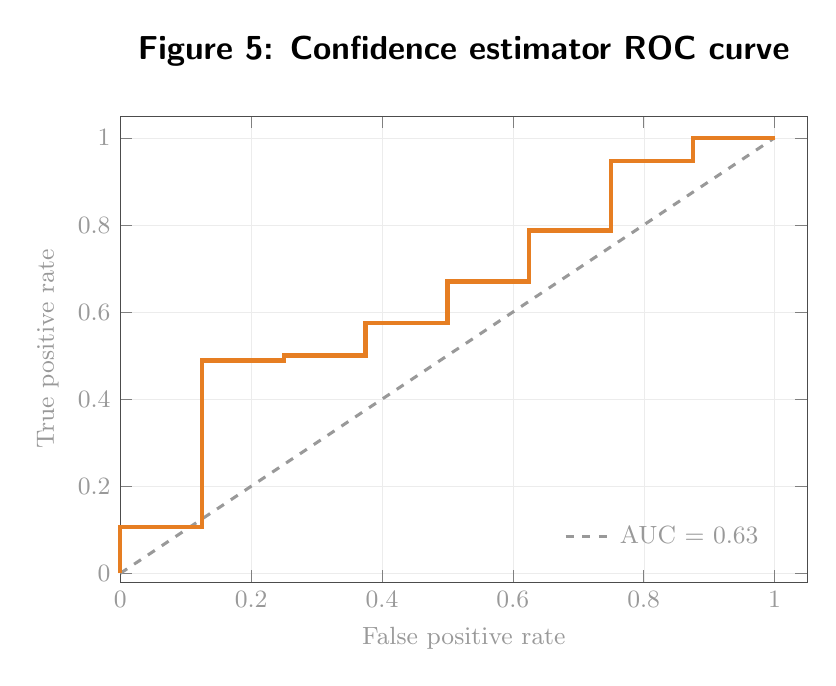
\begin{tikzpicture}
\begin{axis}[
    width=0.85\textwidth, height=7.5cm,
    title={\large Figure 5: Confidence estimator ROC curve},
    title style={at={(0.5,1.05)}, anchor=south, font=\sffamily\bfseries},
    xlabel={False positive rate},
    ylabel={True positive rate},
    xmin=0, xmax=1.05,
    ymin=-0.02, ymax=1.05,
    xtick={0, 0.2, 0.4, 0.6, 0.8, 1.0},
    ytick={0, 0.2, 0.4, 0.6, 0.8, 1.0},
    grid=both,
    grid style={line width=.1pt, draw=gray!15},
    axis line style={black!70},
    tick label style={font=\small\color{gray!80}, /pgf/number format/fixed, /pgf/number format/precision=1},
    label style={font=\small\color{gray!80}},
    legend style={at={(0.95,0.05)}, anchor=south east, draw=none, fill=none, font=\small\color{gray!80}},
    clip=false
]
% Diagonal random baseline
\addplot [gray!80, dashed, line width=1.1pt, domain=0:1] {x};

% ROC staircase - Refined to match the 8-step logic (1/8 = 0.125)
\addplot [myorange, line width=1.6pt, const plot] coordinates {
    (0.000, 0.000)
    (0.000, 0.106)
    (0.125, 0.106)
    (0.125, 0.489)
    (0.250, 0.489)
    (0.250, 0.500)
    (0.375, 0.500)
    (0.375, 0.575)
    (0.500, 0.575)
    (0.500, 0.670)
    (0.625, 0.670)
    (0.625, 0.787)
    (0.750, 0.787)
    (0.750, 0.947)
    (0.875, 0.947)
    (0.875, 1.000)
    (1.000, 1.000)
};

% Legend/Label at bottom right
\addlegendentry{AUC = 0.63}

\end{axis}
\end{tikzpicture}
\caption{ROC curve for the turn-aware confidence estimator (AUC = 0.634). The dashed diagonal represents the random baseline (AUC = 0.500). $N = 102$ labeled turns (94 correct, 8 incorrect).}
\end{figure}
% =============================================================
\section{Discussion}

\subsection{The Query Anchoring Finding}
A key observation from our deployment is that despite measurable retrieval similarity degradation across
turns, our system maintained high accuracy throughout the data collection period. We attribute this to the
\textbf{query anchoring mechanism}: the guardrail model maintains the original query throughout all reasoning
turns, preventing the semantic drift that would otherwise cause correctness degradation. This represents an
accidental discovery --- in building a robust tutoring system, we inadvertently implemented a mitigation for
the degradation phenomenon we later studied.

\subsection{Implications for RAG Evaluation}
Existing benchmarks (BEIR, TriviaQA, NaturalQuestions) all assume single-turn retrieval and cannot capture
the context accumulation effects we document. We argue that agentic RAG evaluation requires: (1)
multi-turn sessions with at least 3 reasoning turns; (2) retrieval quality measurement at each turn
independently; (3) degradation rate as a first-class metric; and (4) sessions where earlier retrieved passages
are topically adjacent but not directly relevant to later sub-queries.

\subsection{Implications for System Design}
\textbf{Context window management.} Selectively drop retrieved passages from earlier turns when their relevance
to the current sub-query falls below a threshold.

\textbf{Turn-aware keyword generation.} Sub-query generation should explicitly re-anchor to the original input
query at each turn. Our query anchoring mechanism demonstrates this is practical and effective.

\textbf{Retrieval confidence monitoring.} A simple context length threshold (AUROC = 0.695) may be sufficient for
practical deployment, requiring no human labels or complex parameter fitting.

\subsection{Limitations}
\textbf{Closed-source LLM.} Our deployment uses Gemini 2.5 Pro. We cannot directly analyze attention weights or
verify the attention head saturation hypothesis. Future work with open-weight models would directly address
this gap.

\textbf{Single domain.} Our data is from mathematics tutoring. Mathematical problems have specific multi-step
structure that may produce different degradation patterns than other domains. Replication in QA, code
generation, and scientific reasoning is needed.

\textbf{Modest degradation magnitude.} The 6.6\% retrieval decline is modest compared to what might be
expected in open-domain settings, partly attributable to our query anchoring mechanism and the constrained
mathematical domain.

\textbf{Correctness label coverage.} Human correctness labels are available for only 18.5\% of turns. The high
system accuracy means correctness degradation may be underrepresented in labels.

\textbf{Single system.} Our findings come from one production system. Multi-system studies are needed to
establish the generality of the degradation pattern.

% =============================================================
\section{Conclusion}
We have presented a systematic empirical study of multi-turn retrieval degradation in a production agentic
RAG system. Across 150 multi-turn sessions (550 turn observations) from a deployed mathematics tutoring
system, we document: (1) a 6.6\% decline in mean retrieval relevance between turn 1 and turn 4 ($p <
0.0001$); (2) a strong negative correlation between context length and retrieval quality ($r = -0.283$, $p <
0.0001$); and (3) keyword drift as a compounding factor ($0.328 \to 0.315$).

We introduce a lightweight turn-aware confidence estimator as a proof-of-concept (AUROC = 0.634), and
find that context length alone is the dominant predictor (AUROC = 0.695). We also report the query
anchoring mechanism as an effective mitigation strategy. These findings carry two concrete implications:
single-turn RAG benchmarks must be supplemented with multi-turn agentic protocols; and context window
management, turn-aware keyword generation, and retrieval confidence monitoring can mitigate degradation
in production systems today.

\bigskip

\noindent\textbf{References}

\begin{hangparas}{2em}{1}
Asai, A., Wu, Z., Wang, Y., Sil, A., and Hajishirzi, H. (2023). Self-RAG: Learning to retrieve, generate, and critique through
     self-reflection. \textit{ICLR 2024}.

Hayashi, K., Kamigaito, H., Kouda, S., and Watanabe, T. (2025). IterKey: Iterative keyword generation with LLMs for
    enhanced retrieval augmented generation. \textit{COLM 2025}.

Jeong, S., Baek, J., Cho, S., Hwang, S. J., and Park, J. C. (2023). Adaptive-RAG: Learning to adapt retrieval-augmented
    large language models through question complexity. \textit{NAACL 2024}.

Jiang, Z., Xu, F. F., Gao, L., et al. (2023). Active retrieval augmented generation. \textit{EMNLP 2023}.

Karpukhin, V., Oguz, B., Min, S., Lewis, P., et al. (2020). Dense passage retrieval for open-domain question answering.
    \textit{EMNLP 2020}.

Kurihara, K., Mita, M., Zhang, P., Sasaki, S., Ishigami, R., and Okazaki, N. (2025). LCTG Bench: LLM controlled text
     generation benchmark. \textit{arXiv:2501.15875}.

Lewis, P., Perez, E., Piktus, A., Petroni, F., et al. (2020). Retrieval-augmented generation for knowledge-intensive NLP tasks.
    \textit{NeurIPS 33}, 9459--9474.

Liu, N. F., Lin, K., Hewitt, J., et al. (2023). Lost in the middle: How language models use long contexts.
    \textit{TACL 12}, 157--173.

Ma, Y. and Okazaki, N. (2026). From interpretability to performance: Optimizing retrieval heads for long-context language
    models. \textit{arXiv:2601.11020}.

Okazaki, N., Hattori, K., Hirai, S., et al. (2024). Building a large Japanese web corpus for large language models.
    \textit{COLM 2024}.

Ozaki, S., Kato, Y., Feng, S., et al. (2025). Understanding the impact of confidence in retrieval augmented generation:
     A case study in the medical domain. \textit{BioNLP 2025}.

Wei, J., Wang, X., Schuurmans, D., et al. (2022). Chain-of-thought prompting elicits reasoning in large language models.
    \textit{NeurIPS 35}.

Yan, S., Gu, J., Zhu, Y., and Ling, Z. (2024). Corrective retrieval augmented generation. \textit{arXiv:2401.15884}.

Yao, S., Zhao, J., Yu, D., et al. (2023). ReAct: Synergizing reasoning and acting in language models. \textit{ICLR 2023}.

Yoshikawa, H. and Okazaki, N. (2023). Selective-LAMA: Selective prediction for confidence-aware evaluation of language
    models. \textit{Findings of EACL 2023}.
\end{hangparas}

\appendix
\renewcommand{\thesection}{Appendix \Alph{section}}

\section{Logging Implementation}
The per-turn logging system was implemented as a TypeScript service (\texttt{logger.ts}) integrated into the
production Gemini API service layer. Each call to \texttt{generateSolution()} logs the following fields after the API
response:
\begin{verbatim}
interface TurnLog {
  sessionId: string           // Random session identifier
  turnNumber: number          // 1-indexed turn within session
  subQuery: string            // First 300 chars of sub-query
  groundingChunkCount: number // From groundingMetadata
  contextTokenCount: number   // From usageMetadata.totalTokenCount
  usedWebSearch: boolean      // Whether Google Search was triggered
  retrievalTier: number       // 1=TF-IDF, 2=KB, 3=Web
  similarityScore: number     // Cosine similarity of top chunk
  anchoringEnabled: boolean   // Whether query anchoring was active
  problemType: string         // algebra/calculus/geometry/statistics
  timestamp: string           // ISO 8601 timestamp
  wasCorrect?: boolean        // From human feedback (when available)
}
\end{verbatim}
Logs are stored in browser localStorage under key \texttt{rag\_research\_logs} and exported as JSON via a
download interface. Session boundaries are determined by new question submission --- each question
initiates a new \texttt{sessionId} automatically via \texttt{resetSession()}.

\section{Parameter Details}
Parameters $\alpha = 0.18$ and $\beta = 0.09$ in the confidence estimator were selected based on the theoretical
relationship between turn number decay and context length penalty in our system. $C_{\mathrm{baseline}} = 482$ tokens
represents the empirically measured mean turn-1 context length across all 150 sessions. The estimator
requires only three observable signals ($t$, $|C|$, $g$) available from any agentic RAG system's API metadata,
making it deployment-agnostic.

\end{document}